% DO NOT COMPILE THIS FILE DIRECTLY!
% This is included by the other .tex files.

%\colorlet{punct}{red!60!black}
%\definecolor{background}{HTML}{EEEEEE}
%\definecolor{delim}{RGB}{20,105,176}
%\colorlet{numb}{magenta!60!black}

\begin{frame}[t,plain]
\titlepage
\end{frame}

\begin{frame}[fragile]
    \frametitle{Viper - Main ideas}
    \begin{quote}
        Viper is a {\bf binary analysis and management framework}. Its
        fundamental objective is to provide a solution to {\bf easily organize}
        your collection of {\bf malware} and {\bf exploit samples} as well as your
        collection of {\bf scripts} you created or found over the time to
        facilitate your daily research. Think of it as a {\bf Metasploit for malware
        researchers}: it provides a terminal interface that you can use to {\bf store},
        {\bf search} and {\bf analyze} arbitrary files with and a framework to
        {\bf easily create plugins} of any sort.
    \end{quote}
\end{frame}


\begin{frame}[fragile]
    \frametitle{Viper}
    \begin{itemize}
        \item {\bf Solid CLI}
        \item Plenty of modules (PE files, *office, ELF, APK, ...)
        \item Connection to {\bf 3rd party services} (MISP, VirusTotal, cuckoo)
        \item Connectors to {\bf 3rd party tools} (IDA, radare)
        \item {\bf Locale storage} of your own zoo
        \item Django interface is available (I've been told)
    \end{itemize}
\end{frame}

\begin{frame}[fragile]
    \frametitle{Viper}
    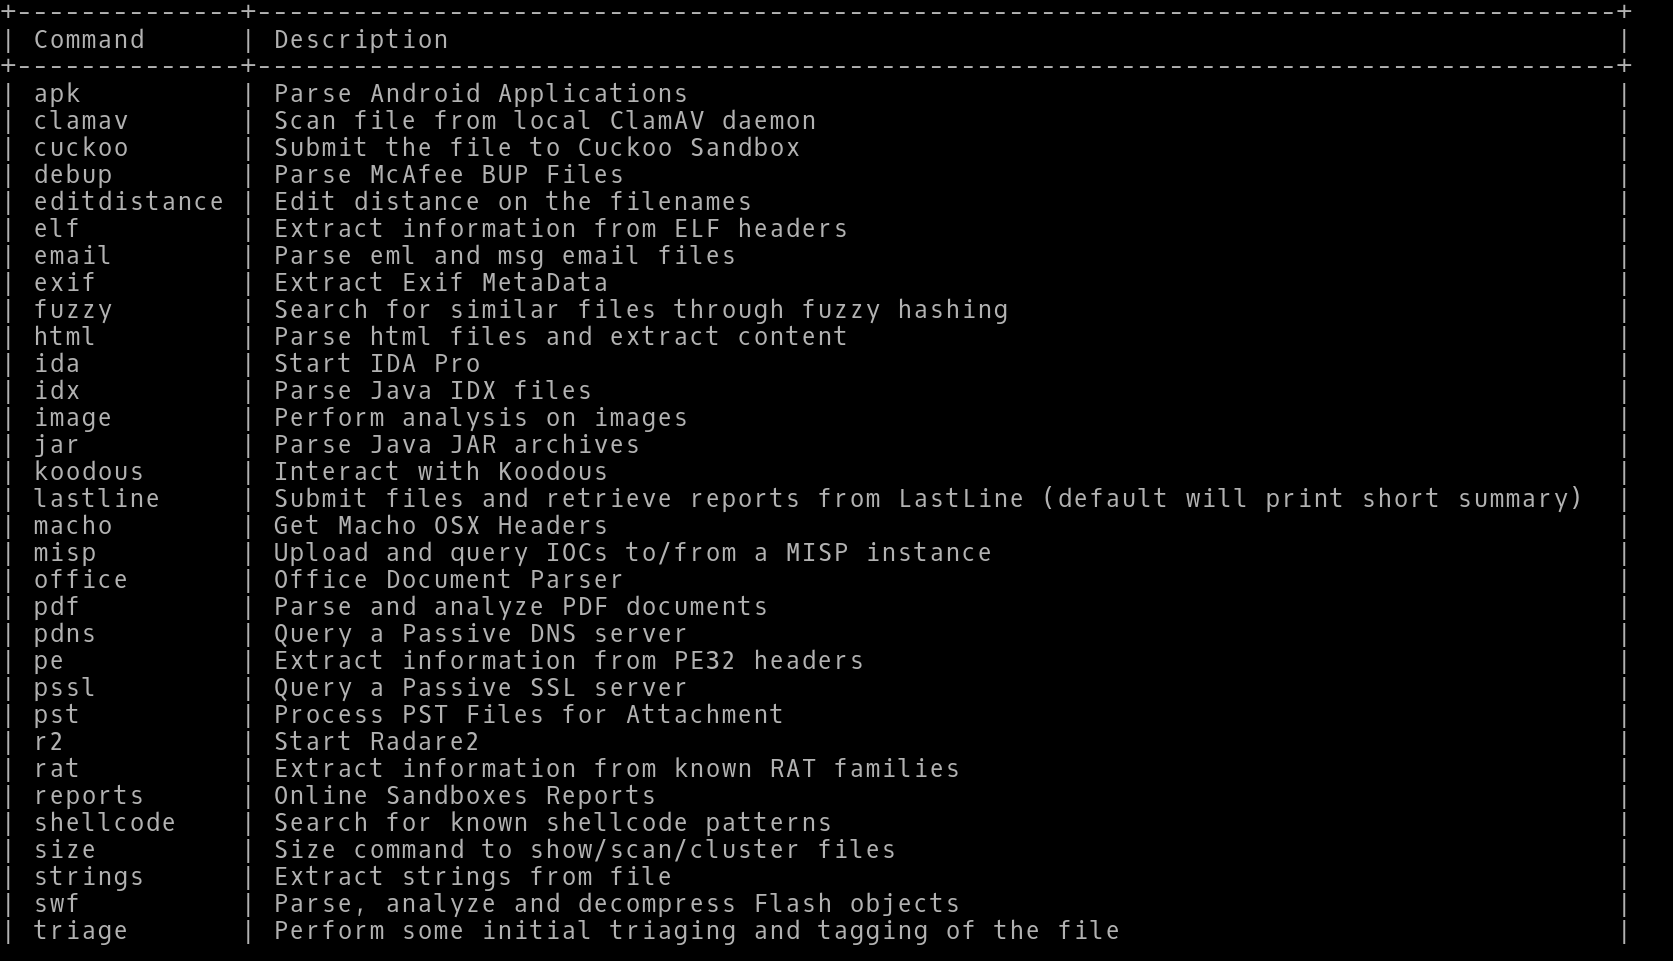
\includegraphics[scale=0.27]{modules.png}
\end{frame}


\begin{frame}[fragile]{PyMISP \& Viper}
    \begin{itemize}
        \item Full featured {\bf CLI for MISP}
        \item {\bf Remote storage} of your zoo
        \item Search / {\bf Cross check with VirusTotal}
        \item Create / Update / Show / Publish Event
        \item Download / Upload Samples
        \item Mass export / Upload / Download
        \item Get Yara rules
    \end{itemize}
\end{frame}

\begin{frame}[fragile]
    \frametitle{MISP Module}
    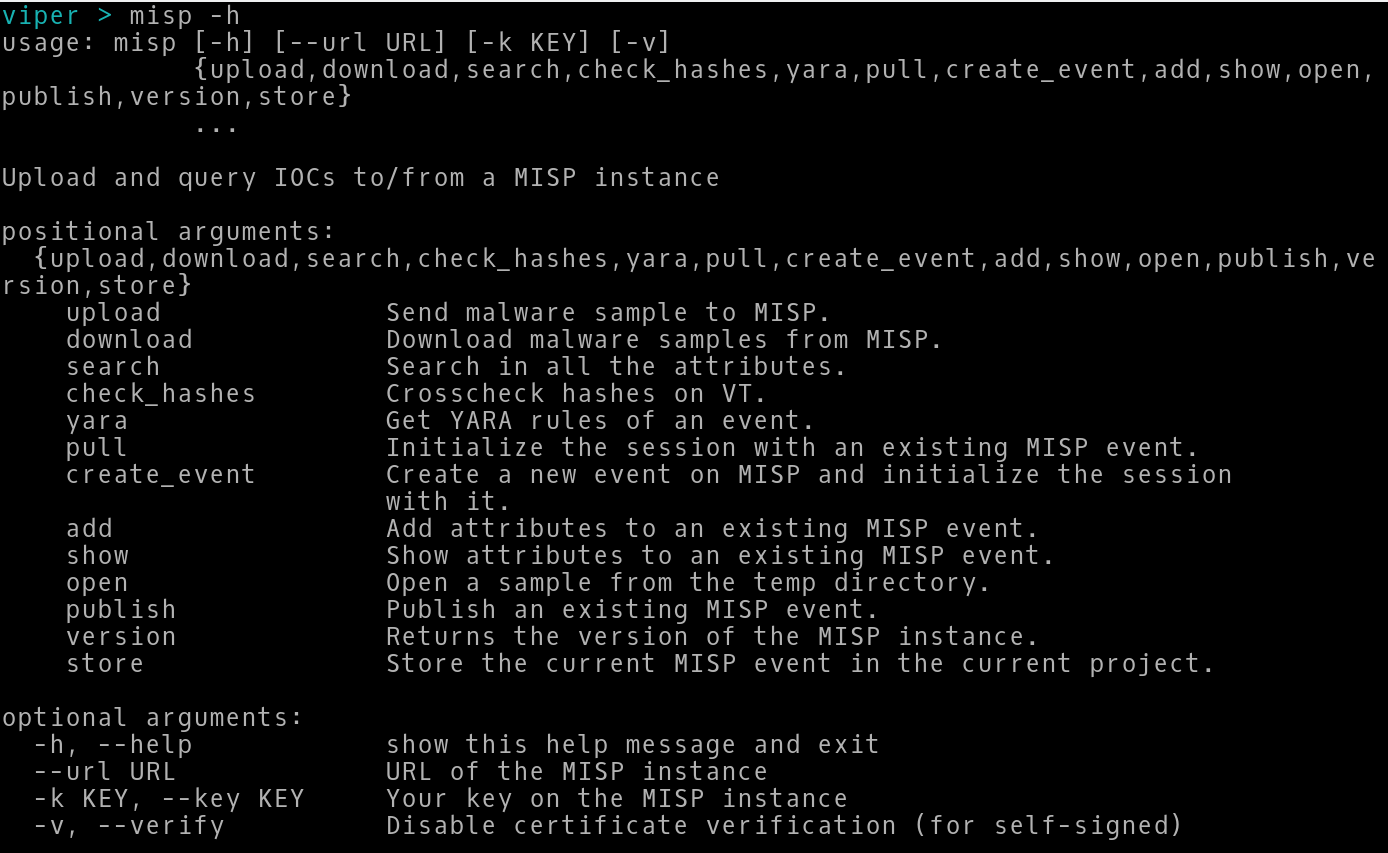
\includegraphics[scale=0.32]{misp.png}
\end{frame}

\begin{frame}[fragile]{Viper \& VT}
    \begin{itemize}
        \item Searches for hashes/ips/domains/URLs from the current MISP event, or download the samples
        \item Download samples from current MISP event
        \item Download all samples from all the MISP events of the current session
    \end{itemize}
\end{frame}

\begin{frame}[fragile]
    \frametitle{VirusTotal Module}
    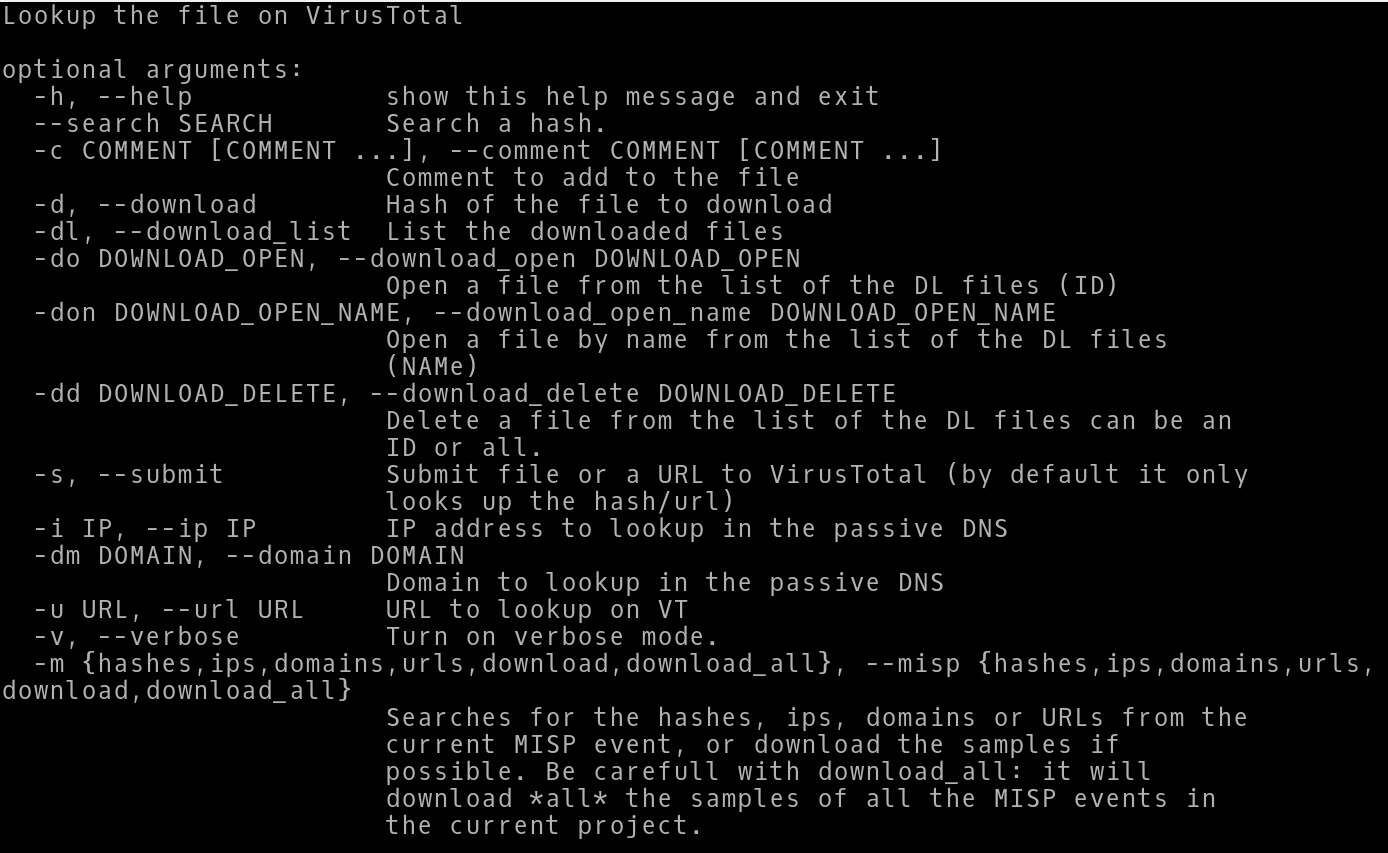
\includegraphics[scale=0.32]{vt.png}
\end{frame}

\begin{frame}[fragile]
    \frametitle{Extra features}
    \begin{itemize}
        \item Link to a MISP event
        \item Local storage of the MISP event
        \item On the fly cross-check of MISP atributes with 3rd party services
        \item Never leaving your CLI!
    \end{itemize}
\end{frame}

\begin{frame}[fragile]{Other modules}
    \begin{itemize}
        \item Fully featured CLI for {\bf Passive SSL}
        \item Fully featured CLI for {\bf Passive DNS}
        \item Can launch Radare2 or IDA
    \end{itemize}
\end{frame}

\begin{frame}[fragile]
    \frametitle{Passive SSL}
    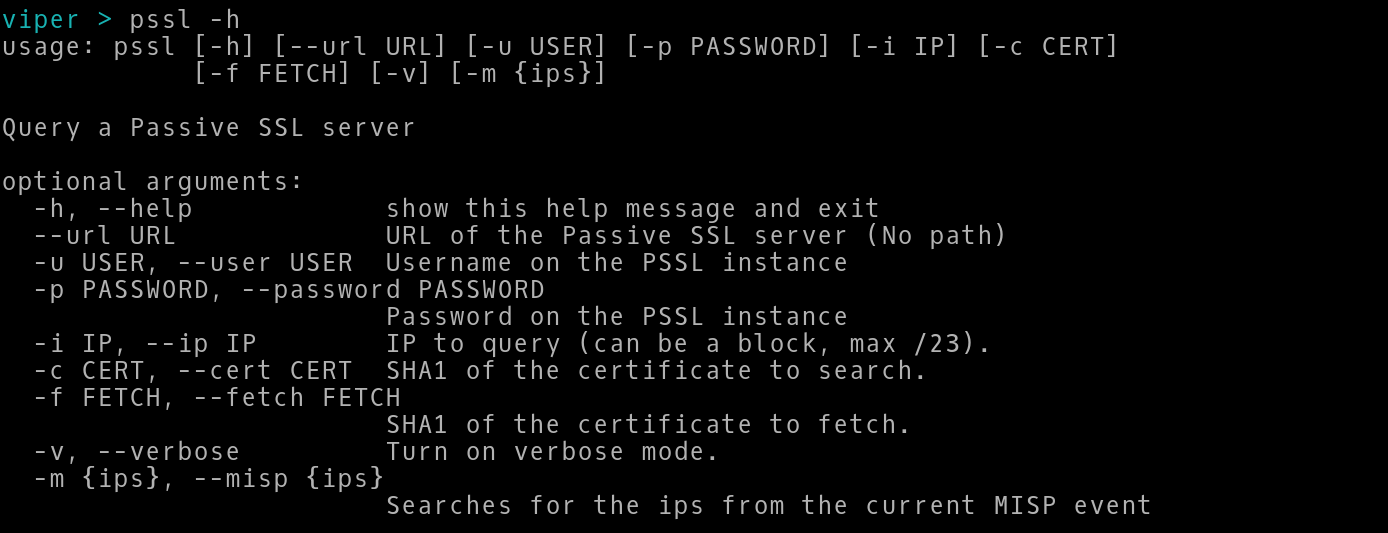
\includegraphics[scale=0.32]{pssl.png}
\end{frame}

\begin{frame}[fragile]
    \frametitle{Passive DNS}
    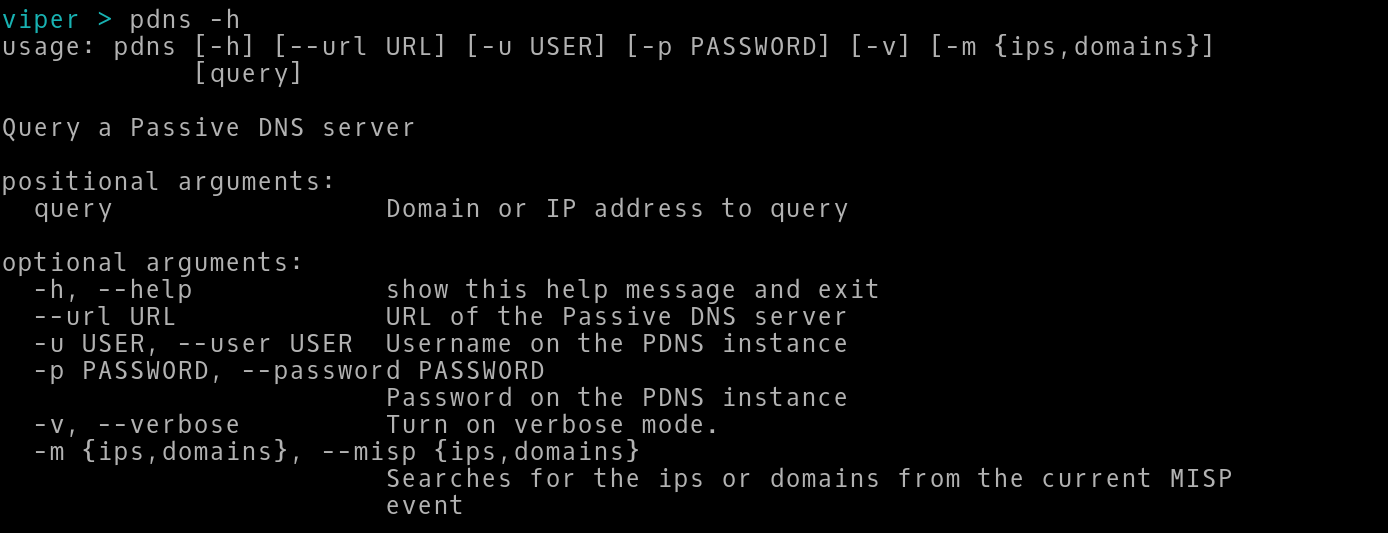
\includegraphics[scale=0.32]{pdns.png}
\end{frame}

\begin{frame}[t,fragile] {Q\&A}

\includegraphics[scale=0.5]{misplogo.pdf}
\begin{itemize}
        \item \url{https://github.com/MISP/PyMISP}
        \item \url{https://github.com/MISP/}
        \item \url{https://github.com/viper-framework/viper}
        \item We welcome new functionalities and pull requests.
\end{itemize}

\end{frame}

